\documentclass{article}

% 导入宏包
\usepackage{fancyhdr}
\usepackage{ctex}
\usepackage{listings}
\usepackage{graphicx}
\usepackage[a4paper, body={18cm,22cm}]{geometry}
\usepackage{amsmath,amsthm,amssymb,amstext,wasysym,enumerate,graphicx}
\usepackage{float,abstract,booktabs,indentfirst,amsmath}
\usepackage{array}
\usepackage{multirow}
\usepackage{url}
\usepackage{diagbox}
\usepackage{enumitem}
\usepackage{xcolor}
\usepackage{makecell}
\usepackage{tikz}
\usepackage{tcolorbox}
\usetikzlibrary{positioning, arrows.meta}
\usepackage[bookmarks=true, colorlinks, citecolor=blue, linkcolor=black]{hyperref}


% 设置段落
\renewcommand\arraystretch{1.4}
\setlength{\parindent}{2em}
\setCJKmonofont{黑体}

% 设置高亮文字
\newtcbox{\mybox}[1][red]
{on line, arc = 0pt, outer arc = 0pt,
	colback = #1!10!white, colframe = #1!50!black,
	boxsep = 0pt, left = 1pt, right = 1pt, top = 2pt, bottom = 2pt,
	boxrule = 0pt, bottomrule = 1pt, toprule = 1pt}

% 配置代码显示
\lstset{
	xleftmargin = 3em,
	xrightmargin = 3em,
	aboveskip = 1em,
	backgroundcolor = \color{white},
	basicstyle = \small\ttfamily,
	rulesepcolor = \color{gray},
	breaklines = true,
	numbers = left,
	numberstyle = \small,
	numbersep = -14pt,
	keywordstyle = \color{purple}\bfseries,
	commentstyle = \color{green!60!black}, % 修改注释颜色
	stringstyle = \color{red!60!green!90!blue!90},
	morekeywords = {ASSERT, int64_t, uint32_t},
	moreemph = {ASSERT, NULL},
	emphstyle = \color{red}\bfseries,
	moreemph = [2]{int64\_t, uint32\_t, tid\_t, uint8\_t, int16\_t, uint16\_t, int32\_t, size\_t, bool},
	emphstyle = [2]\color{purple}\bfseries,
	frame = shadowbox,
	showspaces = false,
	columns = fixed
	morecomment = [l][\color{green!60!black}]{+}, % 设置以+开头的代码行为绿色
}

%--------------------页眉--------------------%

\pagestyle{fancy}
\fancyhead[L]{}
\fancyhead[R]{}
\fancyhead[C]{华东师范大学软件工程学院实验报告}
\fancyfoot[C]{-\thepage-}
\renewcommand{\headrulewidth}{1.5pt}

%--------------------标题--------------------%

\begin{document}
	\begin{center}
		{\Large{\textbf{\heiti 华东师范大学软件工程学院实验报告}}}
		\begin{table}[htb]
			\flushleft
			\begin{tabular}{p{0.4\linewidth}p{0.27\linewidth}p{0.28\linewidth}}\\
				\textbf{实验课程}:数据库系统及其应用实践  & \textbf{年级}:2023级       & \textbf{实验成绩}:  \\
				\textbf{实验名称}:Lab-02 & \textbf{姓名}:顾翌炜         &                 \\
				\textbf{实验编号}:Lab-02     & \textbf{学号}:10235101527 & \textbf{实验日期}:2025/03/26  \\
				\textbf{指导教师}:姚俊杰     & \textbf{组号}:01            & \textbf{实验时间}:2课时  \\ 
			\end{tabular}
		\end{table}
	\end{center}
	\rule{\textwidth}{2pt}
	
	\section{实验目的}
	本实验旨在通过 JDBC(Java Database Connectivity)技术,实现 Java 应用程序与 MySQL 数据库的交互。通过本实验,学生将掌握以下内容:
	\begin{itemize}
		\item 了解 JDBC 的基本概念和原理。
		\item 学习如何使用 JDBC 连接数据库。
		\item 练习 SQL 语句的编写和在 Java 中执行 SQL 查询。
		\item 掌握使用 PreparedStatement 进行安全查询。
		\item 通过编写 Java 代码,实现对数据库的增、删、改、查等操作。
		\item 计算学生的 GPA,并提高对数据库应用的实际能力。
	\end{itemize}
	
	\section{实验要求}
	为了顺利完成本实验,学生需要满足以下要求:
	\begin{itemize}
		\item 熟悉 Java 语言基础,掌握面向对象编程思想。
		\item 了解基本的 SQL 语法,包括 SELECT、INSERT、UPDATE、DELETE 等操作。
		\item 安装并配置 MySQL 数据库,创建实验所需的数据表。
		\item 安装 JDK 并配置 Java 开发环境,确保能够编写和运行 Java 程序。
		\item 下载并正确引用 MySQL JDBC 驱动(Jar 包)。
		\item 编写 Java 代码,实现用户登录、查询学生信息、查询课程信息及计算 GPA 等功能。
		\item 代码需具有较好的可读性,采用异常处理机制,确保系统的稳定性和安全性。
	\end{itemize}
	
	\section{实验过程记录}
	
	\subsection{下载 Java SE}
	
	为了使用 JDBC 连接 MySQL 数据库,我们需要先安装 Java SE(Java Platform, Standard Edition)。本实验使用 Java SE 8 及以上版本。以下是下载和安装步骤:
	
	\subsubsection{访问 Oracle 官方网站}
	首先,打开浏览器,进入 Oracle Java 官方下载页面:
	
	\begin{center}
		\url{https://www.oracle.com/java/technologies/javase-downloads.html}
	\end{center}
	
	\subsubsection{选择 Java SE 版本}
	
	\begin{itemize}
		\item 点击 \textbf{JDK 下载},选择适用于操作系统(Windows/macOS/Linux)的版本。
	\end{itemize}
	
	\subsubsection{下载并安装 JDK}
	\begin{enumerate}
		\item 下载 JDK 安装包后,运行安装程序,并按照默认选项完成安装。
		\item 安装完成后,确认 JDK 目录,例如:
		
	\end{enumerate}
	
	\subsubsection{配置环境变量(Windows 系统)}
	\begin{enumerate}
		\item 右键“此电脑” → “属性” → “高级系统设置” → “环境变量”。
		\item 在 \textbf{系统变量} 中找到 \texttt{Path},点击“编辑”,添加 JDK 的 \texttt{bin} 目录
		\item 新建 \texttt{JAVA\_HOME} 变量,值为 JDK 安装路径
	\end{enumerate}
	
	\subsubsection{验证安装}
	打开终端或命令提示符,输入:
	\begin{verbatim}
		java -version
	\end{verbatim}
	若正确显示 Java 版本信息,则安装成功。
	
	\begin{figure}[H]
		\centering
		\begin{minipage}[b]{0.45\textwidth}
			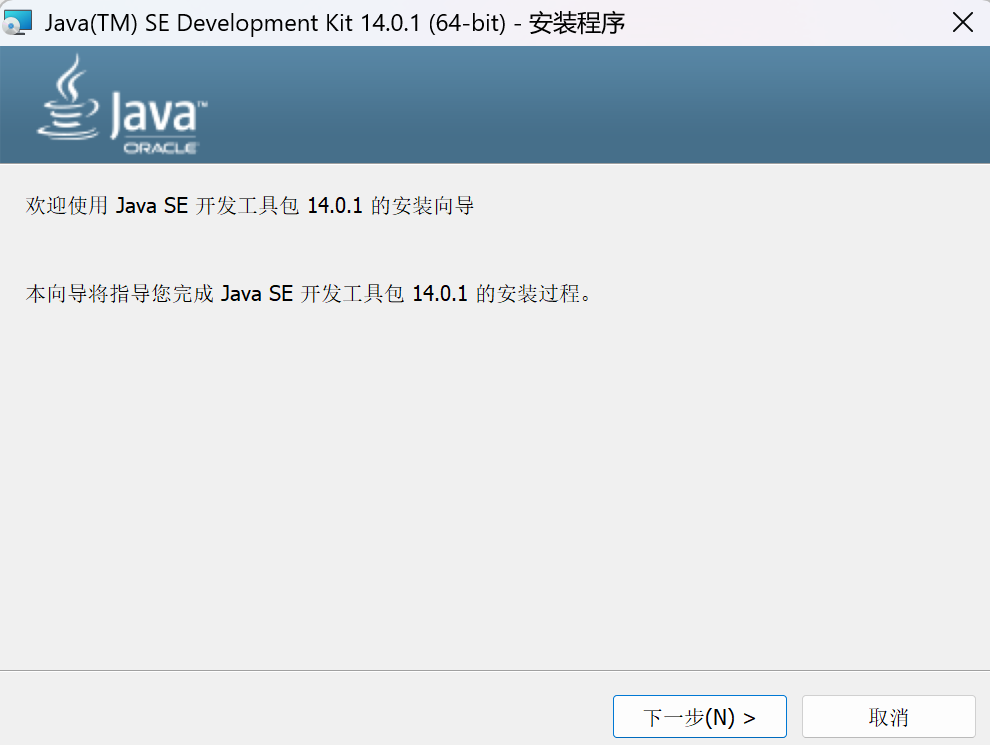
\includegraphics[width=\textwidth]{./images/1.安装Java SE.png}
			\caption{安装Java SE}
		\end{minipage}
		\hfill
		\begin{minipage}[b]{0.45\textwidth}
			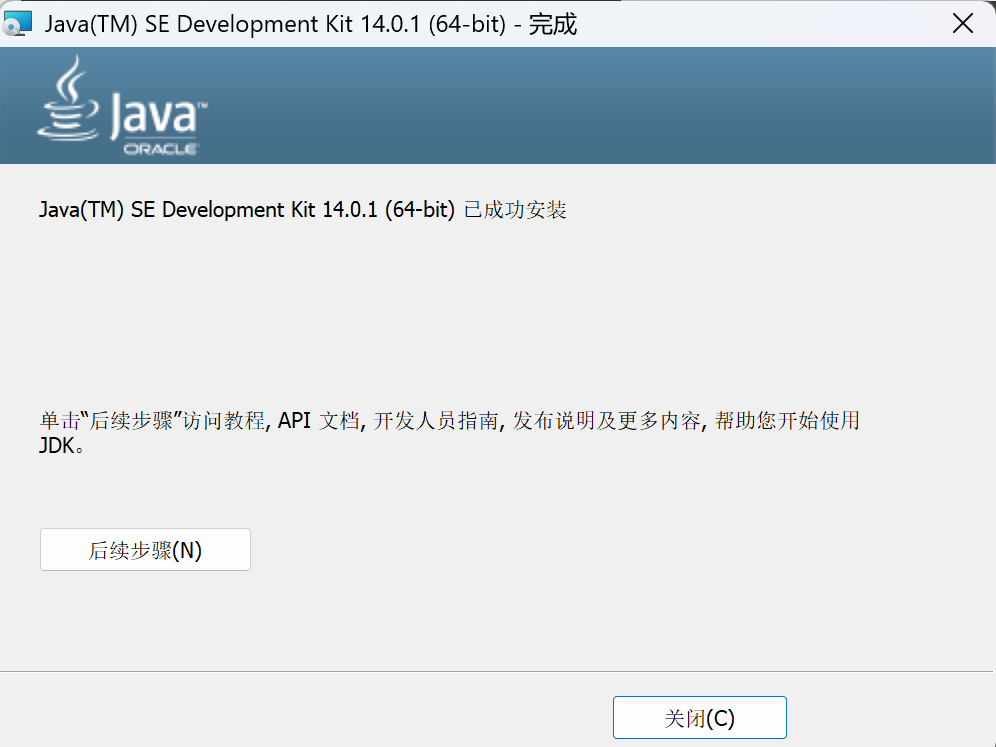
\includegraphics[width=\textwidth]{./images/2.安装Java SE.png}
			\caption{安装Java SE}
		\end{minipage}
	\end{figure}
	
	\subsection{安装JDBC需要的Jar包}
	
	本实验使用 MySQL 数据库,需要 MySQL JDBC 驱动程序(Jar包)以支持 Java 访问数据库。
	
	\begin{enumerate}
		\item 下载老师提供的 JDBC 安装包。
		\item 解压后,获取 \texttt{mysql-connector-java-8.4.0.jar} 文件。
		\item 在 Java 项目中引入该 Jar 包,确保项目能够使用 JDBC 连接数据库。
	\end{enumerate}
	
	\begin{figure}[H]
		\centering
		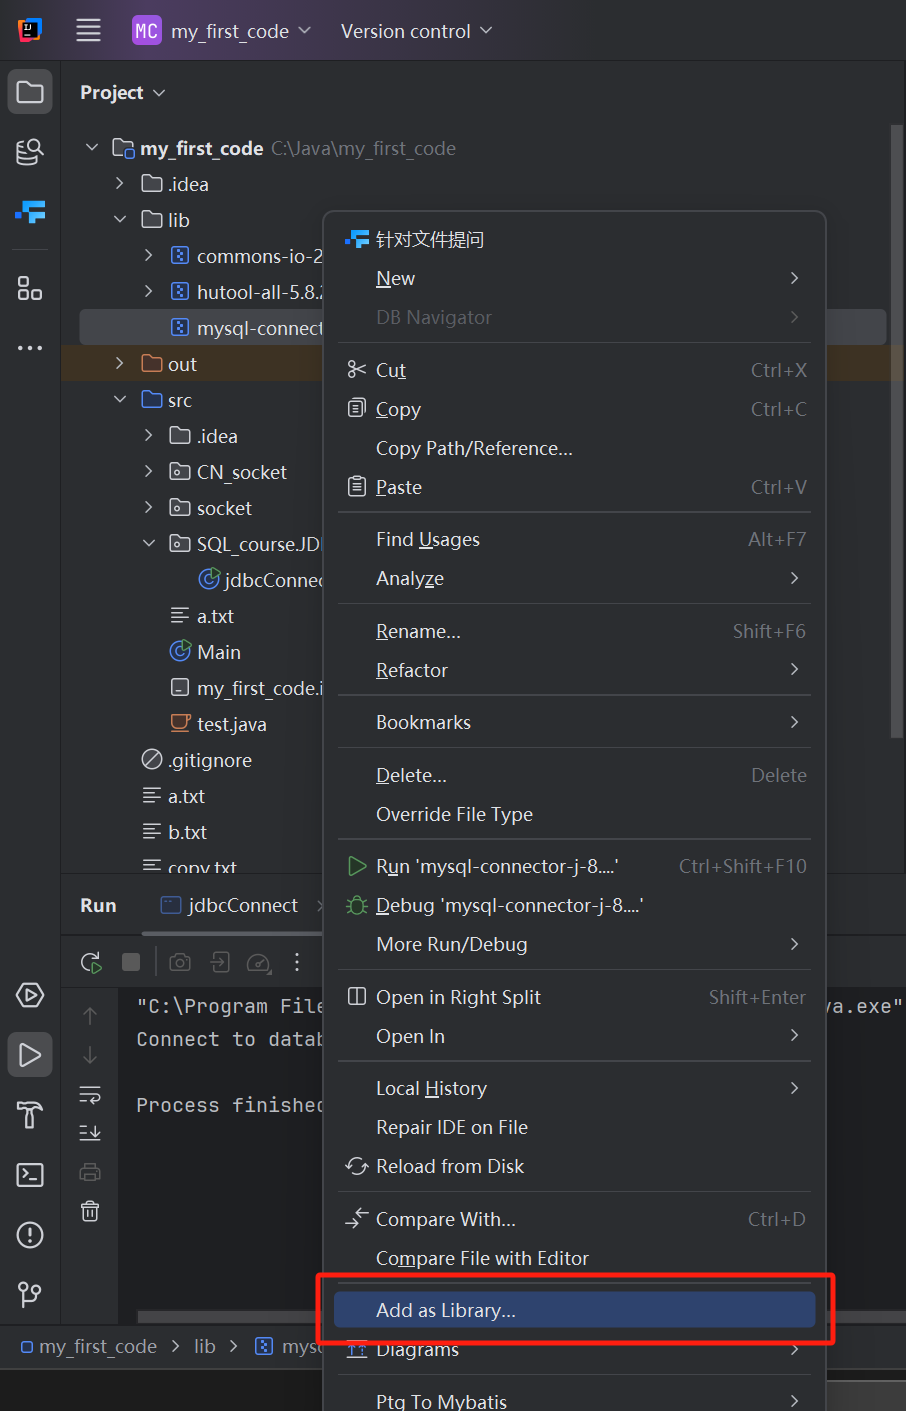
\includegraphics[width=7cm]{./images/3.添加到Library.png}
		\caption{添加到Library}
	\end{figure}
	
	\begin{figure}[H]
		\centering
		\begin{minipage}[b]{0.45\textwidth}
			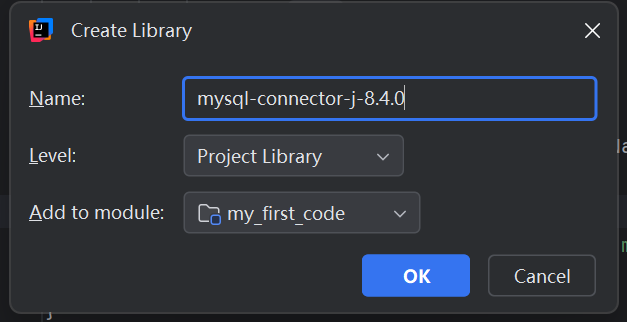
\includegraphics[width=\textwidth]{./images/4.添加到Library.png}
			\caption{Create Library}
		\end{minipage}
		\hfill
		\begin{minipage}[b]{0.45\textwidth}
			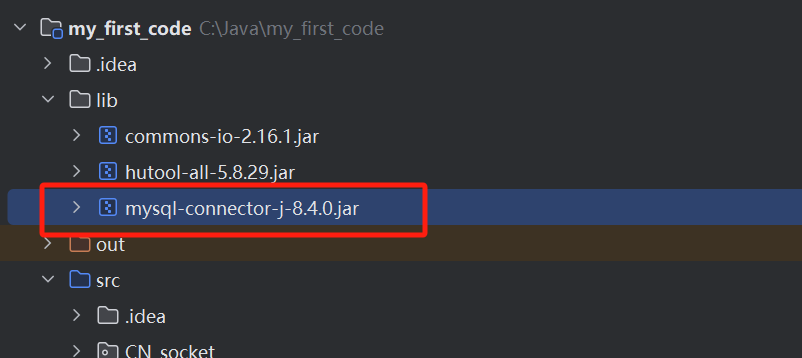
\includegraphics[width=\textwidth]{./images/5.添加到Library.png}
			\caption{添加到Library完毕}
		\end{minipage}
	\end{figure}
	
	\subsection{使用JDBC}
	
	\subsubsection{测试连接}
	
	\begin{lstlisting}[language=java, title=jdbcConnect, tabsize=4]
		package SQL_course.JDBC;
		
		import java.sql.Connection;
		import java.sql.DriverManager;
		
		public class jdbcConnect {
			public static void main(String args[]) {
				Connection c = null;
				try {
					Class.forName("com.mysql.cj.jdbc.Driver");
					c = DriverManager.getConnection(
					"jdbc:mysql://localhost:3306/lab-2_college",
					"root",
					"GUyiwei_)*@@");
				} catch (Exception e) {
					e.printStackTrace();
					System.err.println(e.getClass().getName() + ": " + e.getMessage());
					System.exit(0);
				}
				System.out.println("Connect to database mysql successfully !");
			}
		}
		
	\end{lstlisting}
	
	然后在命令行内输入以下指令:
	
	\verb|java -cp .\lib\mysql-connector-j-8.4.0.jar .\src\SQL_course\JDBC\jdbcConnect.java|
	
	得到以下结果:
	
	\begin{figure}[H]
		\centering
		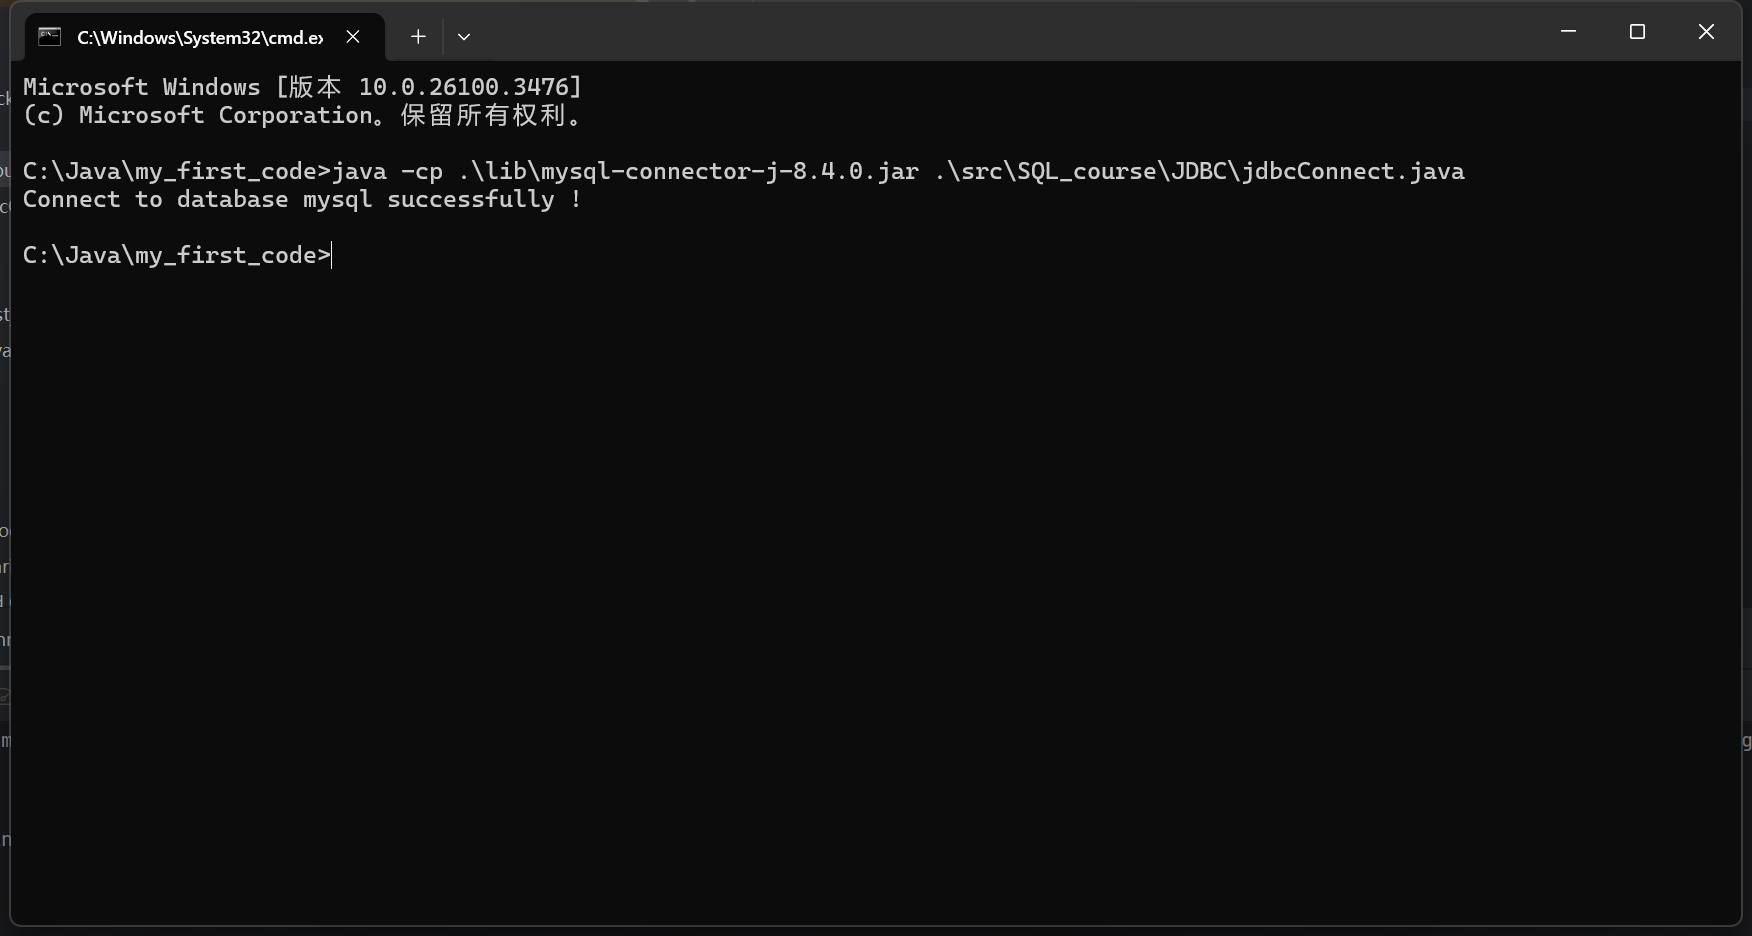
\includegraphics[width=11cm]{./images/6.测试连接.png}
		\caption{测试连接}
	\end{figure}
	
	可以看到:Connect to database mysql successfully !连接成功
	
	\subsubsection{创建表格}
	
	\begin{lstlisting}[language=java, title=jdbcCreate, tabsize=4]
		package SQL_course.JDBC;
		
		import java.sql.Connection;
		import java.sql.DriverManager;
		import java.sql.Statement;
		
		public class jdbcCreate {
			public static void main(String args[]) {
				Connection c = null;
				Statement stmt = null;
				
				try {
					// 加载 MySQL JDBC 驱动
					Class.forName("com.mysql.cj.jdbc.Driver");
					
					// 建立连接
					c = DriverManager.getConnection(
					"jdbc:mysql://localhost:3306/lab-2_college",
					"root",
					"GUyiwei_)*@@"
					);
					System.out.println("Connect to database mysql successfully!");
					
					// 创建 Statement 对象
					stmt = c.createStatement();
					
					// 创建表的 SQL 语句
					String sql = "CREATE TABLE employee " +
					"(id INT, " +
					" name VARCHAR(20) NOT NULL, " +
					" age INT NOT NULL, " +
					" address VARCHAR(50), " +
					" salary REAL, " +
					" PRIMARY KEY (id))";
					
					// 执行创建表的 SQL 语句
					stmt.executeUpdate(sql);
					stmt.close();
					c.close();
					
				} catch (Exception e) {
					// 捕获并打印异常
					System.err.println(e.getClass().getName() + ": " + e.getMessage());
					System.exit(0);
				}
				// 打印成功消息
				System.out.println("Create table company successfully!");
			}
		}
	\end{lstlisting}
	
	然后在命令行内输入以下指令:
	
	\verb|java -cp .\lib\mysql-connector-j-8.4.0.jar .\src\SQL_course\JDBC\jdbcCreate.java|
	
	得到以下结果:
	
	\begin{figure}[H]
		\centering
		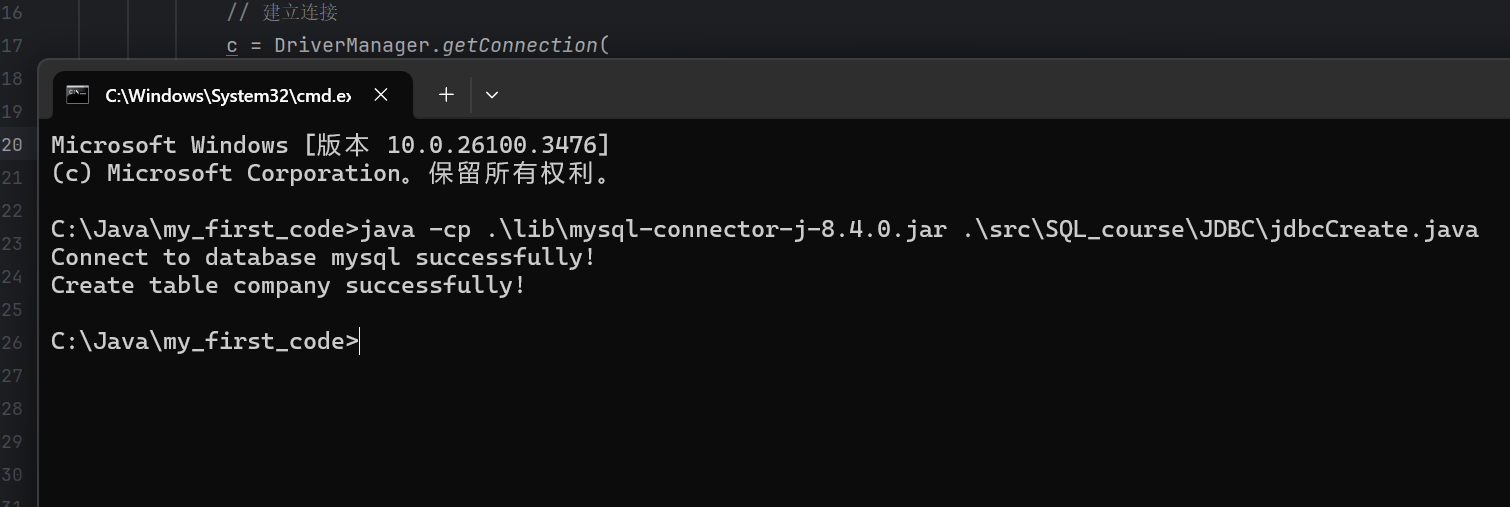
\includegraphics[width=11cm]{./images/7.创建表格.png}
		\caption{创建表格}
	\end{figure}
	
	可以看到:
	
	Connect to database mysql successfully !
	
	Create table company successfully!
	
	创建成功
	
	\subsubsection{插入数据}
	
	\begin{lstlisting}[language=java, title=jdbcInsert, tabsize=4]
		package SQL_course.JDBC;
		
		import java.sql.Connection;
		import java.sql.DriverManager;
		import java.sql.Statement;
		
		public class jdbcInsert {
			public static void main(String args[]) {
				Connection c = null;
				Statement stmt = null;
				
				try {
					// 加载 MySQL JDBC 驱动
					Class.forName("com.mysql.cj.jdbc.Driver");
					
					// 建立连接
					c = DriverManager.getConnection(
					"jdbc:mysql://localhost:3306/lab-2_college",
					"root",
					"GUyiwei_)*@@"
					);
					System.out.println("Connected to the database successfully!");
					
					// 创建 Statement 对象
					stmt = c.createStatement();
					
					// 插入数据的 SQL 语句
					String sql1 = "INSERT INTO employee VALUES (1, 'Gong', 48, '2075 Kongjiang Road', 20000.00);";
					String sql2 = "INSERT INTO employee VALUES (2, 'Luan', 25, '3663 Zhongshan Road(N)', 15000.00);";
					String sql3 = "INSERT INTO employee VALUES (3, 'Hu', 23, '3663 Zhongshan Road(N)', 15000.00);";
					String sql4 = "INSERT INTO employee VALUES (4, 'Jin', 24, '3663 Zhongshan Road(N)', 15000.00);";
					String sql5 = "INSERT INTO employee VALUES (5, 'Yi', 24, '3663 Zhongshan Road(N)', 15000.00);";
					
					// 执行插入数据的 SQL 语句
					stmt.executeUpdate(sql1);
					stmt.executeUpdate(sql2);
					stmt.executeUpdate(sql3);
					stmt.executeUpdate(sql4);
					stmt.executeUpdate(sql5);
					
					stmt.close();
					c.close();
					
					System.out.println("Records inserted successfully!");
					
				} catch (Exception e) {
					// 捕获并打印异常
					System.err.println(e.getClass().getName() + ": " + e.getMessage());
					System.exit(0);
				}
			}
		}
		
	\end{lstlisting}
	
	然后在命令行内输入以下指令:
	
	\verb|java -cp .\lib\mysql-connector-j-8.4.0.jar .\src\SQL_course\JDBC\jdbcInsert.java|
	
	得到以下结果:
	
	\begin{figure}[H]
		\centering
		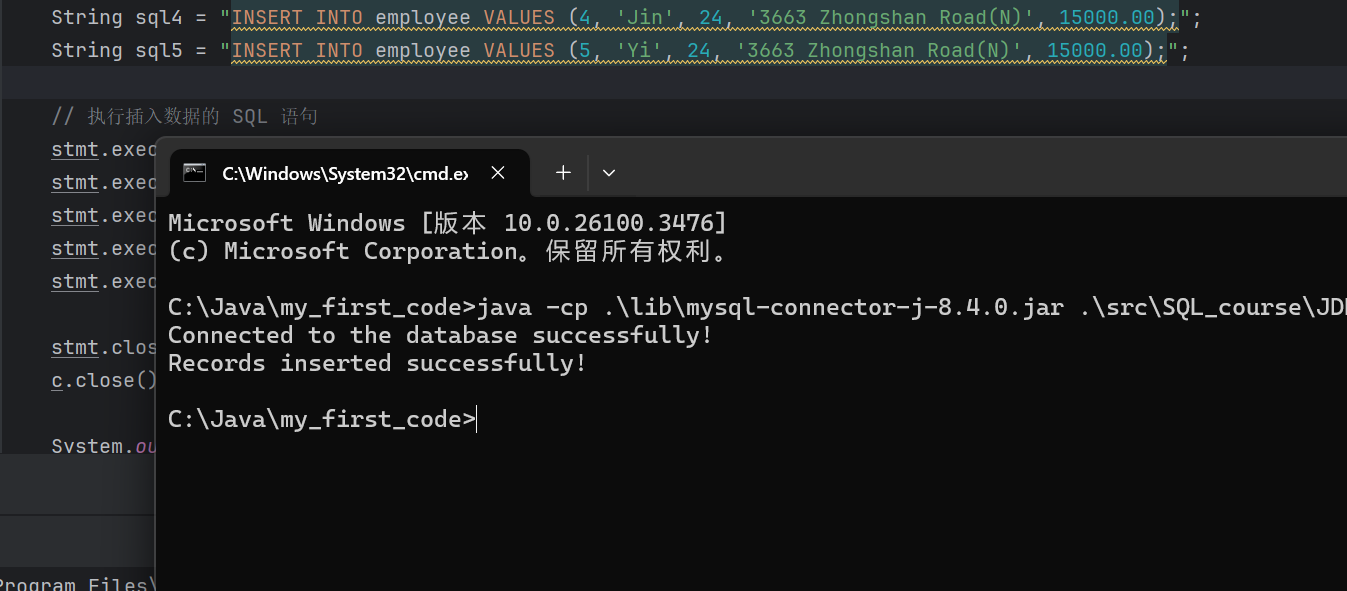
\includegraphics[width=11cm]{./images/8.插入数据.png}
		\caption{插入数据}
	\end{figure}
	
	可以看到:
	
	Connect to database mysql successfully !
	
	Records inserted successfully!
	
	创建成功
	
	我们也可以在数据库里看到新插入的数据,上传成功:
	
	\begin{figure}[H]
		\centering
		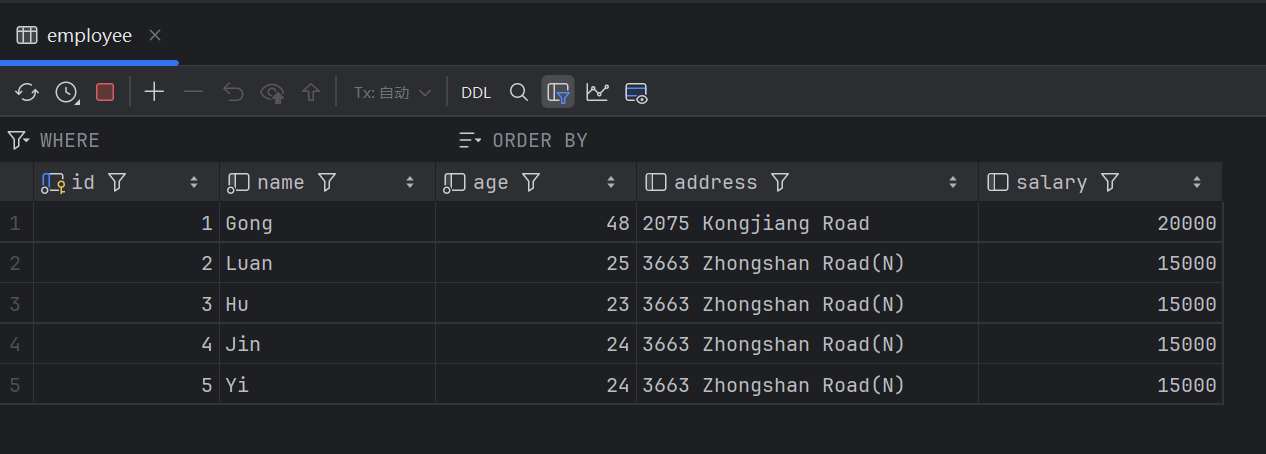
\includegraphics[width=11cm]{./images/9.插入结果.png}
		\caption{插入结果}
	\end{figure}
	
	\subsubsection{查询数据}
	
	\begin{lstlisting}[language=java, title=jdbcSelect, tabsize=4]
		package SQL_course.JDBC;
		
		import java.sql.Connection;
		import java.sql.DriverManager;
		import java.sql.ResultSet;
		import java.sql.Statement;
		
		public class jdbcSelect {
			public static void main(String args[]) {
				Connection c = null;
				Statement stmt = null;
				
				try {
					// 加载 MySQL JDBC 驱动
					Class.forName("com.mysql.cj.jdbc.Driver");
					
					// 建立连接
					c = DriverManager.getConnection(
					"jdbc:mysql://localhost:3306/lab-2_college",
					"root",
					"GUyiwei_)*@@"
					);
					System.out.println("Connect to database mysql successfully!");
					
					// 创建 Statement 对象
					stmt = c.createStatement();
					
					// 查询的 SQL 语句
					String sql = "SELECT * FROM employee";
					
					// 执行查询的 SQL 语句
					ResultSet rs = stmt.executeQuery(sql);
					
					// 处理结果集
					while (rs.next()) {
						int id = rs.getInt("id");
						String name = rs.getString("name");
						int age = rs.getInt("age");
						String address = rs.getString("address");
						double salary = rs.getDouble("salary");
						
						// 打印结果
						System.out.println("ID: " + id);
						System.out.println("Name: " + name);
						System.out.println("Age: " + age);
						System.out.println("Address: " + address);
						System.out.println("Salary: " + salary);
						System.out.println();
					}
					
					// 关闭资源
					rs.close();
					stmt.close();
					c.close();
					
				} catch (Exception e) {
					// 捕获并打印异常
					System.err.println(e.getClass().getName() + ": " + e.getMessage());
					System.exit(0);
				}
				// 打印成功消息
				System.out.println("Select operation successfully!");
			}
		}
		
	\end{lstlisting}
	
	然后在命令行内输入以下指令:
	
	\verb|java -cp .\lib\mysql-connector-j-8.4.0.jar .\src\SQL_course\JDBC\jdbcSelect.java|
	
	得到以下结果:
	
	\begin{figure}[H]
		\centering
		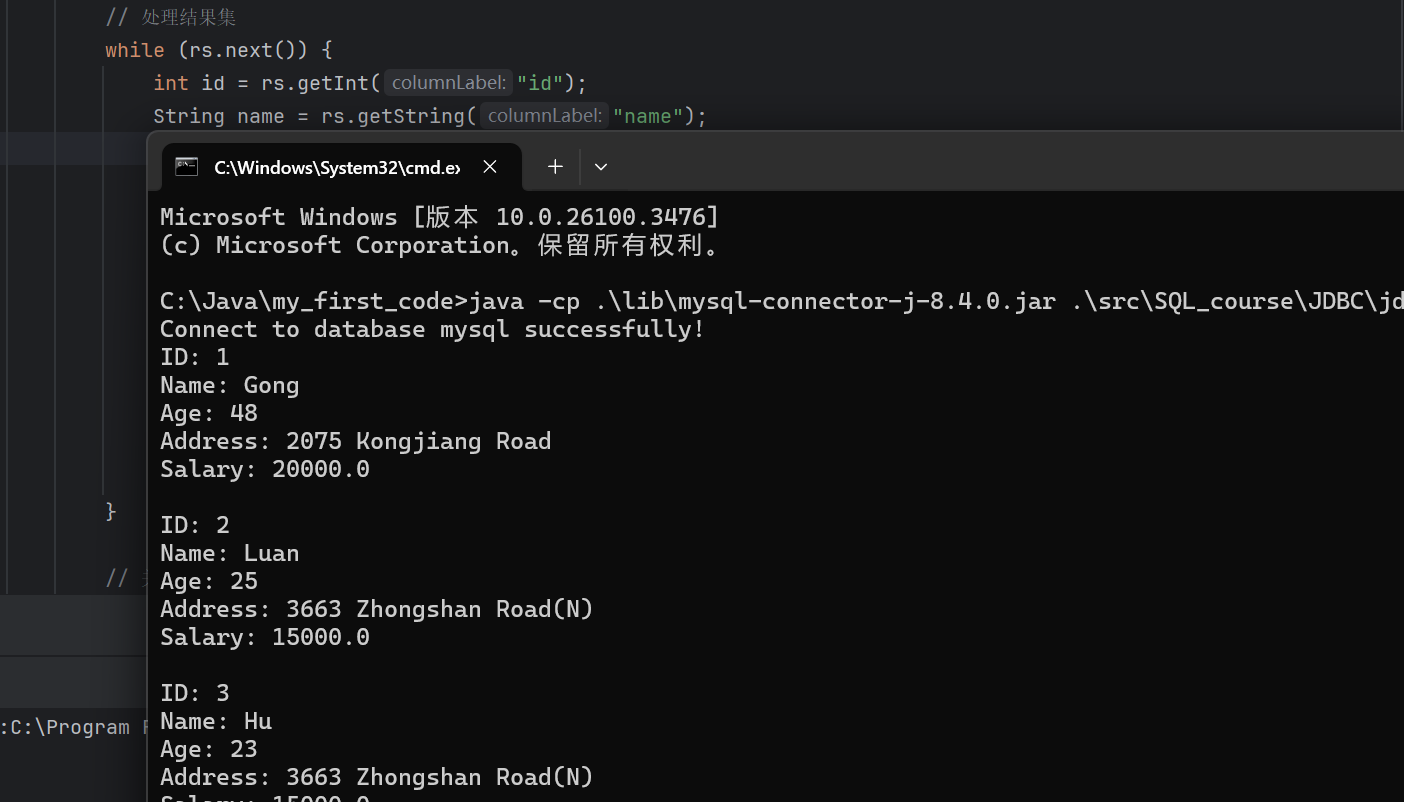
\includegraphics[width=11cm]{./images/10.查询数据.png}
		\caption{查询数据}
	\end{figure}
	
	可以看到:
	
	Connect to database mysql successfully !\\
	ID:1\\
	Name: Gong\\
	Age: 48\\
	Address: 2075 Kongjiang Road\\
	Salary:20000.0\\\\
	ID:2\\
	Name: Luan\\
	Age: 25\\
	Address:3663 Zhongshan Road(N)\\
	Salary: 15000.0\\
	
	···
	
	查询成功
	
	\subsubsection{更新数据}
	
	\begin{lstlisting}[language=java, title=jdbcUpdate, tabsize=4]
		package SQL_course.JDBC;
		
		import java.sql.Connection;
		import java.sql.DriverManager;
		import java.sql.ResultSet;
		import java.sql.Statement;
		
		public class jdbcUpdate {
			public static void main(String args[]) {
				Connection c = null;
				Statement stmt = null;
				
				try {
					// 加载 MySQL JDBC 驱动
					Class.forName("com.mysql.cj.jdbc.Driver");
					
					// 建立连接
					c = DriverManager.getConnection(
					"jdbc:mysql://localhost:3306/lab-2_college",
					"root",
					"GUyiwei_)*@@"
					);
					System.out.println("Connect to database mysql successfully!");
					
					// 创建 Statement 对象
					stmt = c.createStatement();
					
					// 更新的 SQL 语句
					String updateSql = "UPDATE employee SET salary = 50000.00 WHERE id = 1";
					
					// 执行更新的 SQL 语句
					stmt.executeUpdate(updateSql);
					System.out.println("Update operation successfully!");
					
					// 查询的 SQL 语句
					String selectSql = "SELECT * FROM employee";
					
					// 执行查询的 SQL 语句
					ResultSet rs = stmt.executeQuery(selectSql);
					
					// 处理结果集
					while (rs.next()) {
						int id = rs.getInt("id");
						String name = rs.getString("name");
						int age = rs.getInt("age");
						String address = rs.getString("address");
						double salary = rs.getDouble("salary");
						
						// 打印结果
						System.out.println("ID: " + id);
						System.out.println("Name: " + name);
						System.out.println("Age: " + age);
						System.out.println("Address: " + address);
						System.out.println("Salary: " + salary);
						System.out.println();
					}
					
					// 关闭资源
					rs.close();
					stmt.close();
					c.close();
					
				} catch (Exception e) {
					// 捕获并打印异常
					System.err.println(e.getClass().getName() + ": " + e.getMessage());
					System.exit(0);
				}
				// 打印成功消息
				System.out.println("Select operation successfully!");
			}
		}
		
	\end{lstlisting}
	
	然后在命令行内输入以下指令:
	
	\verb|java -cp .\lib\mysql-connector-j-8.4.0.jar .\src\SQL_course\JDBC\jdbcUpdate.java|
	
	得到以下结果:
	
	\begin{figure}[H]
		\centering
		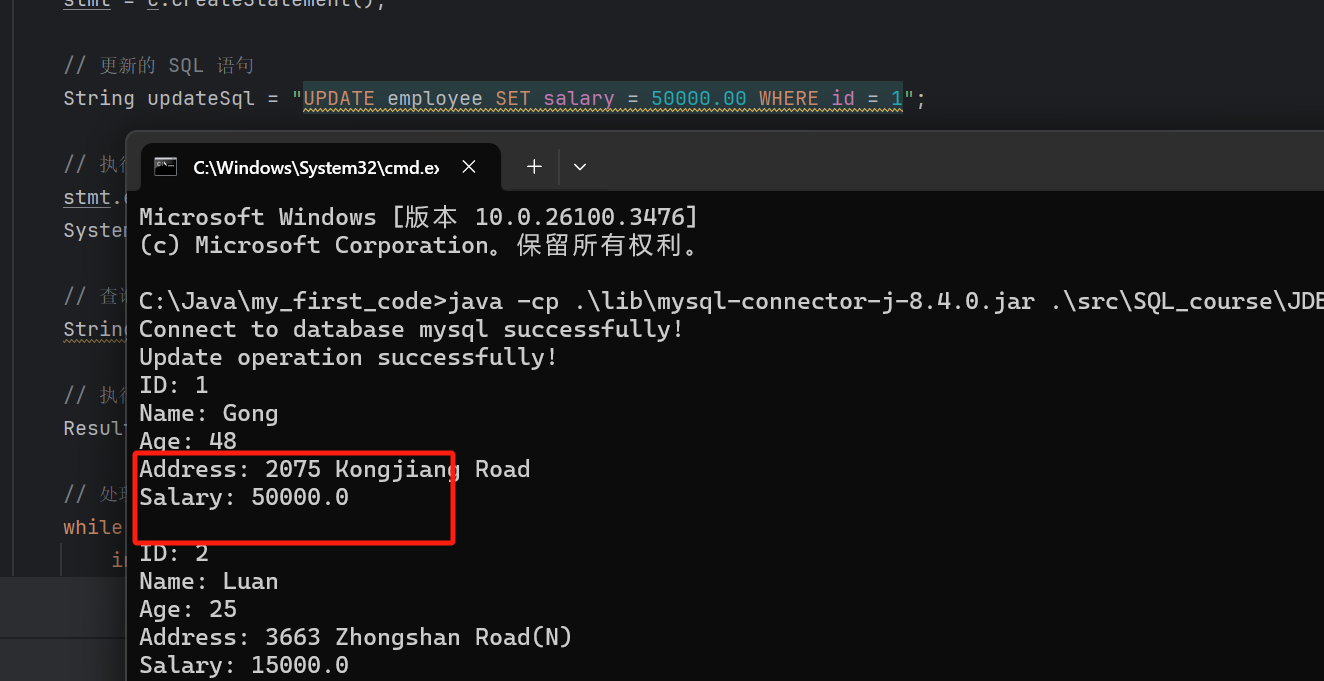
\includegraphics[width=11cm]{./images/11.更新数据.png}
		\caption{更新数据}
	\end{figure}
	
	可以看到:
	
	Connect to database mysql successfully !
	
	且Gong的Salary被更新到50000.0
	
	更新成功
	
	\subsubsection{删除数据}
	
	\begin{lstlisting}[language=java, title=jdbcDelete, tabsize=4]
		package SQL_course.JDBC;
		
		import java.sql.Connection;
		import java.sql.DriverManager;
		import java.sql.ResultSet;
		import java.sql.Statement;
		
		public class jdbcDelete {
			public static void main(String args[]) {
				Connection c = null;
				Statement stmt = null;
				
				try {
					// 加载 MySQL JDBC 驱动
					Class.forName("com.mysql.cj.jdbc.Driver");
					
					// 建立连接
					c = DriverManager.getConnection(
					"jdbc:mysql://localhost:3306/lab-2_college",
					"root",
					"GUyiwei_)*@@"
					);
					System.out.println("Connect to database mysql successfully!");
					
					// 创建 Statement 对象
					stmt = c.createStatement();
					
					// 删除的 SQL 语句
					String deleteSQL = "DELETE FROM employee WHERE ID=2";
					
					// 执行删除的 SQL 语句
					stmt.executeUpdate(deleteSQL);
					System.out.println("Delete operation successfully!");
					
					// 查询的 SQL 语句
					String selectSQL = "SELECT * FROM employee";
					
					// 执行查询的 SQL 语句
					ResultSet rs = stmt.executeQuery(selectSQL);
					
					// 处理结果集
					while (rs.next()) {
						int id = rs.getInt("id");
						String name = rs.getString("name");
						int age = rs.getInt("age");
						String address = rs.getString("address");
						double salary = rs.getDouble("salary");
						
						// 打印结果
						System.out.println("ID: " + id);
						System.out.println("Name: " + name);
						System.out.println("Age: " + age);
						System.out.println("Address: " + address);
						System.out.println("Salary: " + salary);
						System.out.println();
					}
					
					// 关闭资源
					rs.close();
					stmt.close();
					c.close();
					
				} catch (Exception e) {
					// 捕获并打印异常
					System.err.println(e.getClass().getName() + ": " + e.getMessage());
					System.exit(0);
				}
			}
		}
		
	\end{lstlisting}
	
	然后在命令行内输入以下指令:
	
	\verb|java -cp .\lib\mysql-connector-j-8.4.0.jar .\src\SQL_course\JDBC\jdbcDelete.java|
	
	得到以下结果:
	
	\begin{figure}[H]
		\centering
		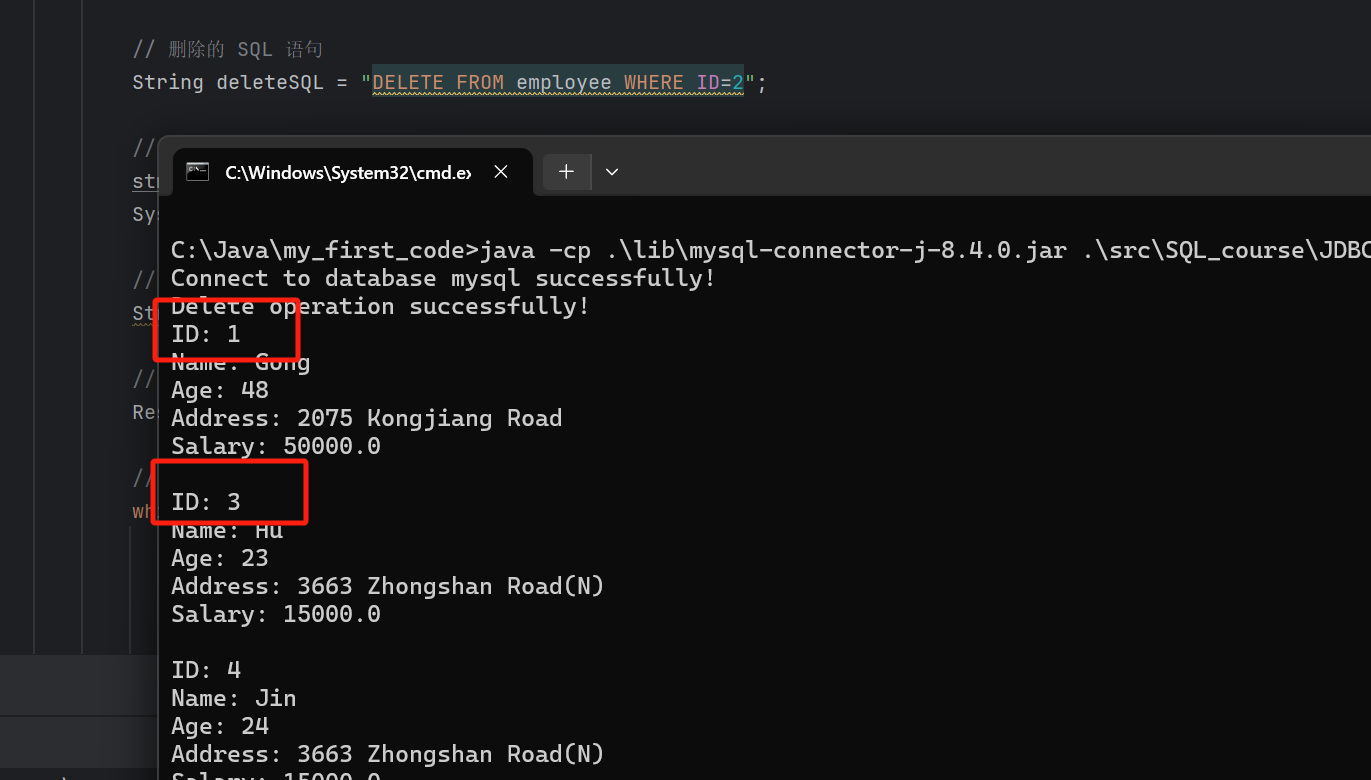
\includegraphics[width=11cm]{./images/12.删除数据.png}
		\caption{删除数据}
	\end{figure}
	
	可以看到:
	
	Connect to database mysql successfully !
	
	且ID为2的数据已经删除
	
	再来数据库内查看:
	
	\begin{figure}[H]
		\centering
		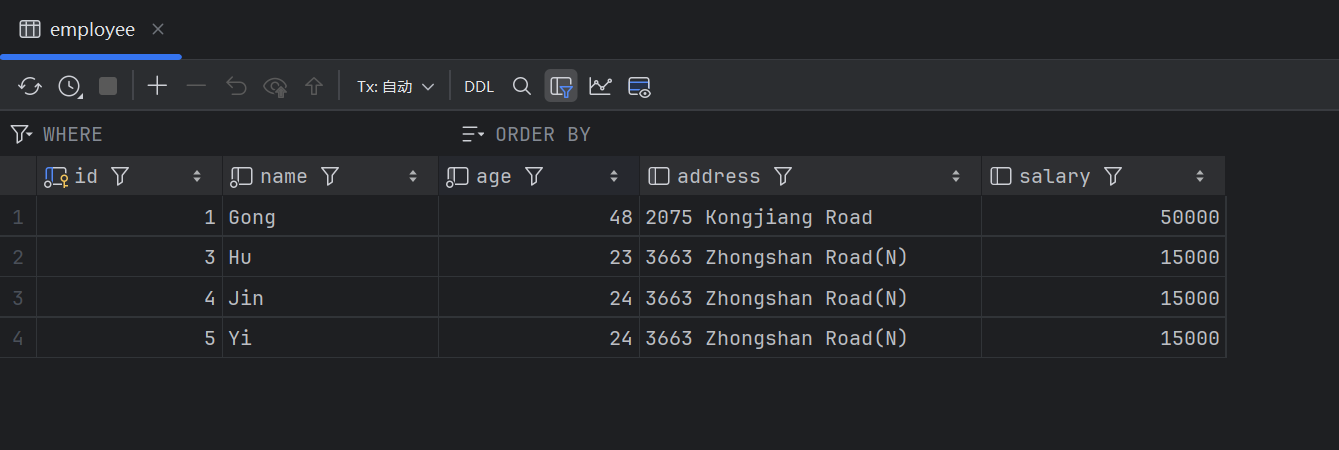
\includegraphics[width=11cm]{./images/13.删除结果.png}
		\caption{删除结果}
	\end{figure}
	
	删除成功
	
	\subsubsection{综合处理}
	
	\begin{lstlisting}[language=java, title=jdbcBatch, tabsize=4]
		package SQL_course.JDBC;
		
		import java.sql.Connection;
		import java.sql.DriverManager;
		import java.sql.PreparedStatement;
		import java.sql.ResultSet;
		import java.sql.SQLException;
		import java.math.BigDecimal;
		
		public class jdbcBatch {
			public static void main(String args[]) {
				Connection c = null;
				PreparedStatement pstmt = null;
				ResultSet rs = null;
				
				try {
					// 加载 MySQL JDBC 驱动
					Class.forName("com.mysql.cj.jdbc.Driver");
					
					// 建立连接
					c = DriverManager.getConnection(
					"jdbc:mysql://localhost:3306/lab-2_college",
					"root",
					"GUyiwei_)*@@"
					);
					System.out.println("Connect to database mysql successfully!");
					
					// 创建 GPA 表的 SQL 语句
					String createTableSQL = "CREATE TABLE GPA (grade CHAR(2), grade_point DECIMAL(3,2))";
					PreparedStatement createTableStmt = c.prepareStatement(createTableSQL);
					createTableStmt.executeUpdate();
					createTableStmt.close();
					System.out.println("Create table GPA successfully!");
					
					// 批量插入数据的 SQL 语句
					String insertSQL = "INSERT INTO GPA (grade, grade_point) VALUES (?, ?)";
					pstmt = c.prepareStatement(insertSQL);
					
					String[] strArray = {"A+", "A", "A-", "B+", "B", "B-", "C+", "C", "C-", "D", "D-", "F"};
					double[] doubleArray = {4.3, 4.0, 3.7, 3.3, 3.0, 2.7, 2.3, 2.0, 1.5, 1.3, 1.0, 0};
					
					for (int i = 0; i < strArray.length; i++) {
						pstmt.setString(1, strArray[i]);
						pstmt.setBigDecimal(2, BigDecimal.valueOf(doubleArray[i]));
						pstmt.addBatch();
					}
					
					pstmt.executeBatch();
					pstmt.close();
					System.out.println("Batch insert into GPA table successfully!");
					
					// 更新数据的 SQL 语句
					String updateSQL = "UPDATE GPA SET grade_point = ? WHERE grade = ?";
					pstmt = c.prepareStatement(updateSQL);
					
					pstmt.executeBatch();
					pstmt.close();
					System.out.println("Batch update into GPA table successfully!");
					
					// 查询的 SQL 语句
					String selectSQL = "SELECT * FROM GPA";
					pstmt = c.prepareStatement(selectSQL);
					rs = pstmt.executeQuery();
					
					// 处理结果集
					while (rs.next()) {
						String grade = rs.getString("grade");
						BigDecimal gradePoint = rs.getBigDecimal("grade_point");
						
						// 打印结果
						System.out.println("Grade: " + grade);
						System.out.println("Grade Point: " + gradePoint);
						System.out.println();
					}
					
					// 关闭资源
					rs.close();
					pstmt.close();
					c.close();
					System.out.println("Select operation successfully!");
					
				} catch (Exception e) {
					// 捕获并打印异常
					System.err.println(e.getClass().getName() + ": " + e.getMessage());
					System.exit(0);
				}
			}
		}
		
	\end{lstlisting}
	
	然后在命令行内输入以下指令:
	
	\verb|java -cp .\lib\mysql-connector-j-8.4.0.jar .\src\SQL_course\JDBC\jdbcBatch.java|
	
	得到以下结果:
	
	\begin{figure}[H]
		\centering
		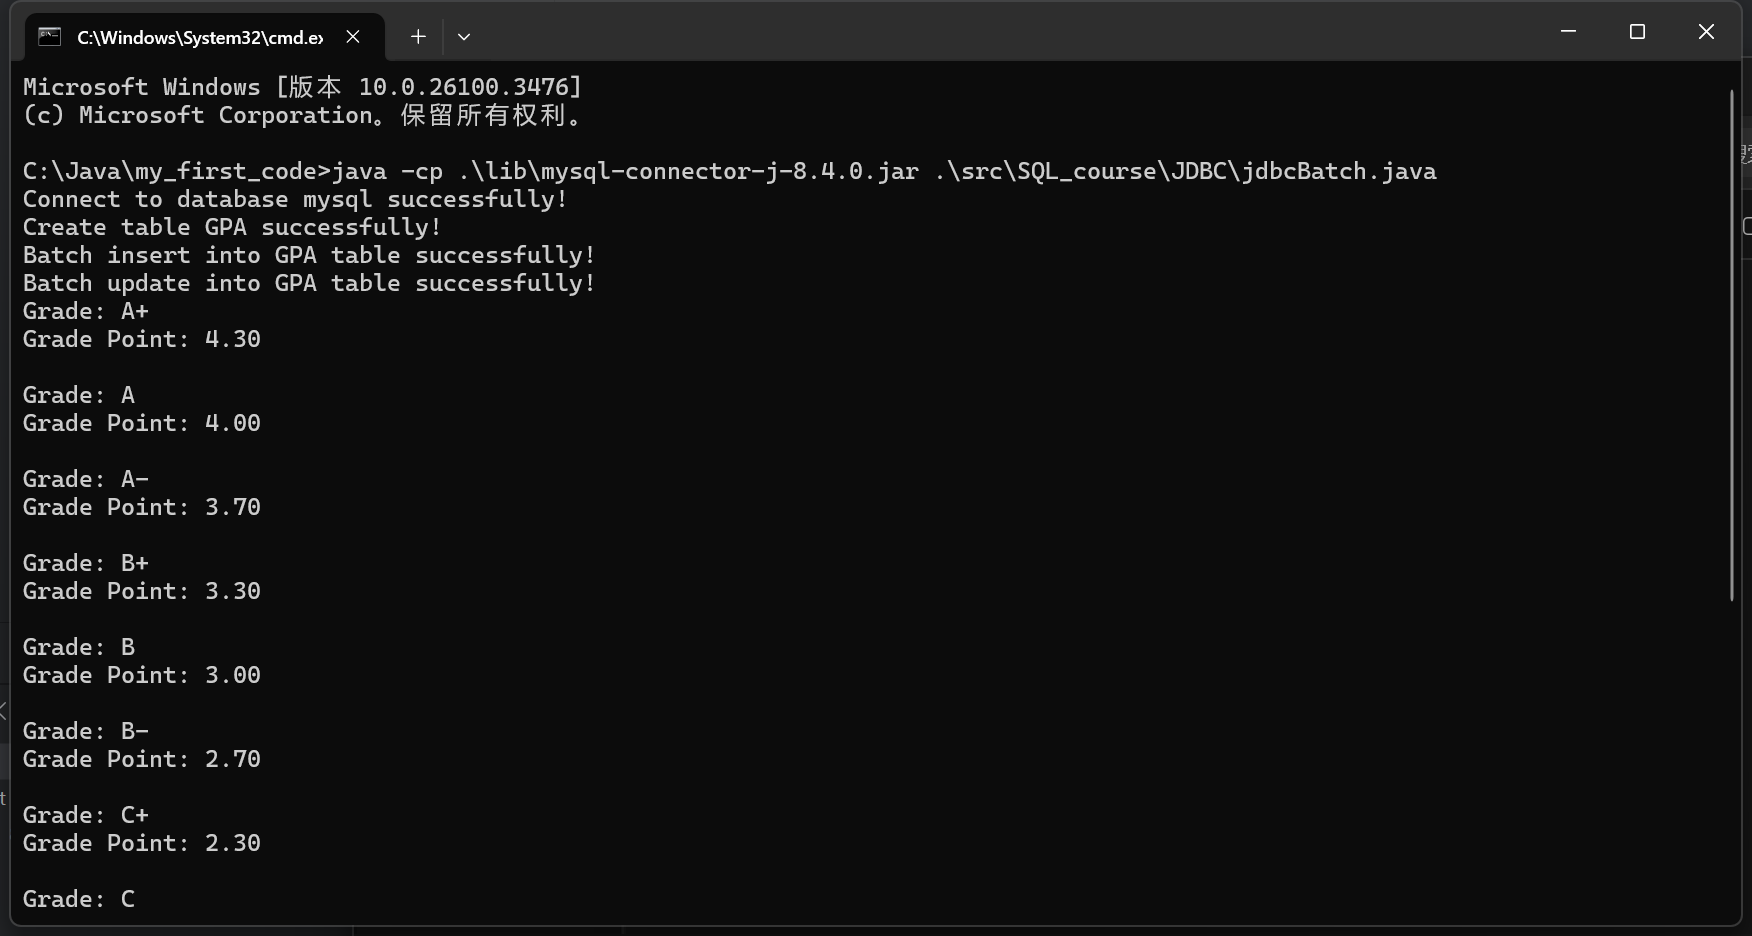
\includegraphics[width=11cm]{./images/14.综合处理.png}
		\caption{综合处理}
	\end{figure}
	
	可以看到:
	
	Connect to database mysql successfully !
	
	且GPA相关的数据已经输入成功
	
	再来数据库内查看:
	
	\begin{figure}[H]
		\centering
		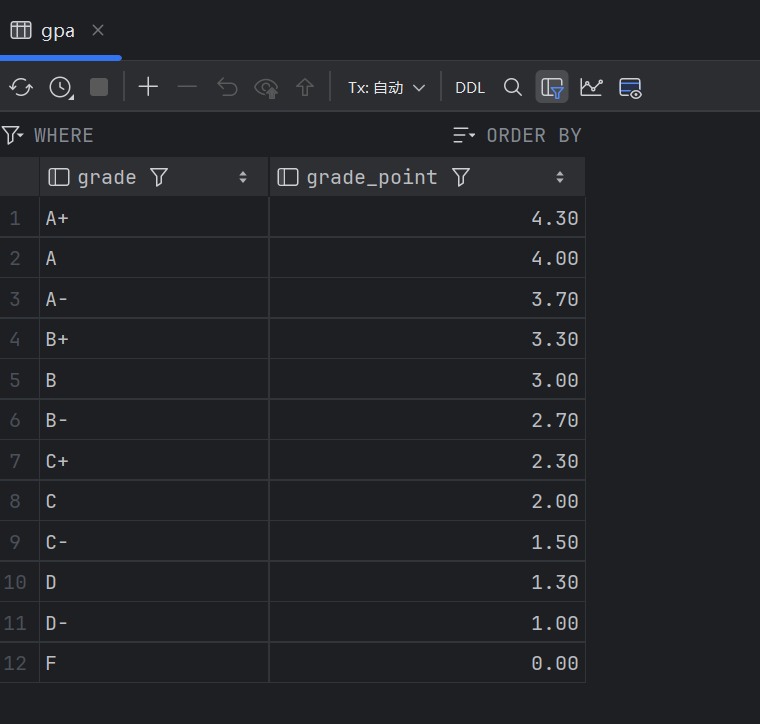
\includegraphics[width=11cm]{./images/15.综合结果.png}
		\caption{综合结果}
	\end{figure}
	
	处理成功
	
	\subsection{JDBC小项目作业}
	
	\begin{tcolorbox}[title = {备注:}, colback = blue!25!white, colframe = blue!75!black]
		以下的实验运行截图中,若无特殊标记,都默认查询Manber(ID: 1000)这位同学的相关课程与绩点信息。
	\end{tcolorbox}
	
	\subsubsection{数据库连接与用户登录}
	\begin{enumerate}
		\item 连接 SQL(实验报告 1)中使用的 \texttt{college} 数据库。
		\item 用户输入登录 ID 和密码,建立数据库连接。
		\item 若连接失败,提示错误信息并允许用户重试。
	\end{enumerate}
	
	\begin{lstlisting}[language=java, title=连接数据库, tabsize=4]
		while (true) {
			try {
				System.out.print("输入数据库用户名: ");
				String user = scanner.nextLine();
				System.out.print("输入数据库密码: ");
				String pass = scanner.nextLine();
				conn = DriverManager.getConnection(URL, user, pass);
				System.out.println("数据库连接成功!");
				break;
			} catch (SQLException e) {
				System.out.println("数据库连接失败,请重试!");
			}
		}
	\end{lstlisting}
	
	以上代码用于建立数据库连接,并提示用户输入用户名和密码进行登录
	
	运行结果如下所示:
	
	\begin{figure}[H]
		\centering
		\begin{minipage}[b]{0.45\textwidth}
			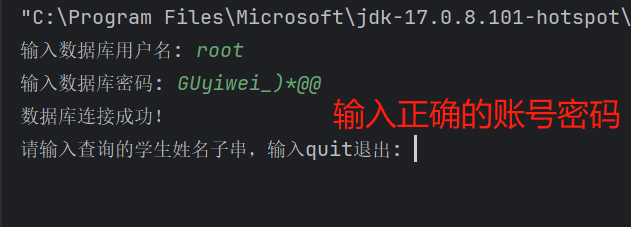
\includegraphics[width=\textwidth]{./images/16.正确登录.png}
			\caption{正确登录}
		\end{minipage}
		\hfill
		\begin{minipage}[b]{0.45\textwidth}
			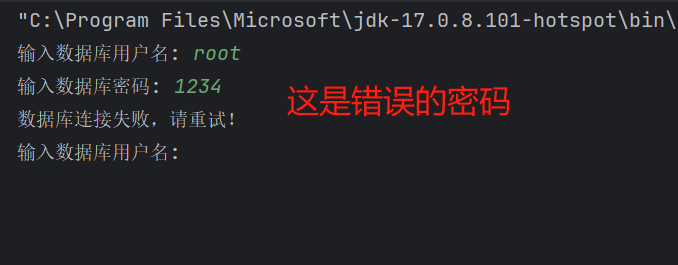
\includegraphics[width=\textwidth]{./images/17.错误登录.png}
			\caption{错误登录}
		\end{minipage}
	\end{figure}
	
	\subsubsection{学生信息查询}
	\begin{enumerate}
		\item 连接成功后,用户输入一个字符串,查询名字中含有该子串的所有学生信息(ID、姓名、院系、总学分)。
		
		\begin{lstlisting}[language=java, title=输入学生姓名, tabsize=4]
			try {
				while (true) {
					System.out.print("请输入查询的学生姓名子串,输入quit退出: ");
					String nameSubstr = scanner.nextLine();
					if (nameSubstr.equals("quit")) {
						break;
					}
					searchStudentsByName(conn, nameSubstr); // 调用函数
				}
			} catch (SQLException e) {
				System.out.println("查询失败: " + e.getMessage());
			}
		\end{lstlisting}
		
		运行结果如下所示:
		
		\begin{figure}[H]
			\centering
			\begin{minipage}[b]{0.45\textwidth}
				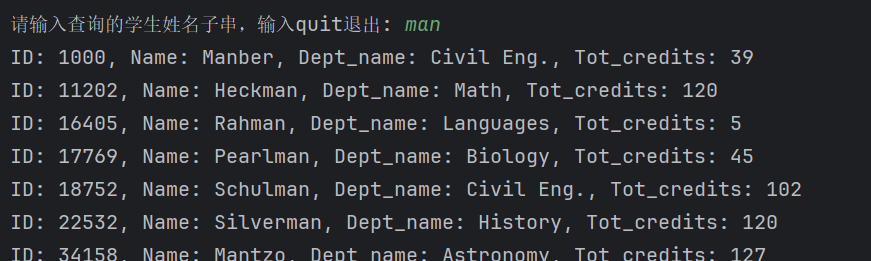
\includegraphics[width=\textwidth]{./images/18.查询子串1.png}
				\caption{查询子串-man}
			\end{minipage}
			\hfill
			\begin{minipage}[b]{0.45\textwidth}
				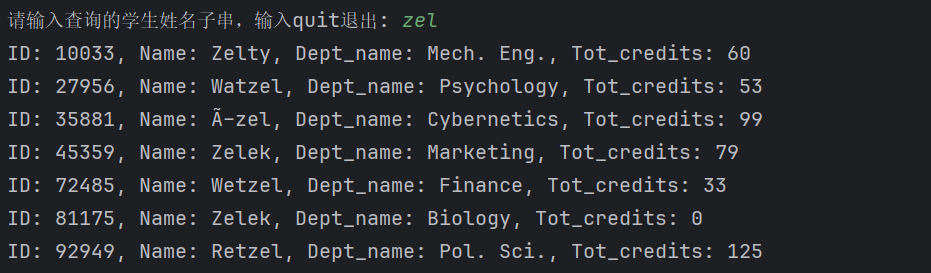
\includegraphics[width=\textwidth]{./images/18.查询子串2.png}
				\caption{查询子串-zel}
			\end{minipage}
		\end{figure}
		
		\item 若查询结果为空,提示用户无相关学生并允许重新输入。
		
		\begin{lstlisting}[language=java, title=查询名字中含有该子串的所有学生信息, tabsize=4]
			private static void searchStudentsByName(Connection conn, String nameSubstr) throws SQLException {
				String query = "SELECT ID, name, dept_name, tot_cred FROM student WHERE name LIKE ?";
				try (PreparedStatement stmt = conn.prepareStatement(query)) {
					stmt.setString(1, "%" + nameSubstr + "%");
					ResultSet rs = stmt.executeQuery();
					boolean found = false;
					while (rs.next()) {
						found = true;
						System.out.println("ID: " + rs.getInt("ID") + ", Name: " + rs.getString("name") + ", Dept_name: " + rs.getString("dept_name") + ", Tot_credits: " + rs.getInt("tot_cred"));
					}
					if (!found) {
						System.out.println("未找到相关学生。");
					} else {
						searchStudentById(conn);
					}
				}
			}
		\end{lstlisting}
		
		\begin{figure}[H]
			\centering
			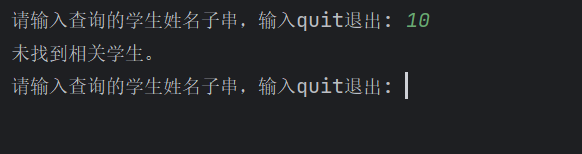
\includegraphics[width=11cm]{./images/19.查询子串错误.png}
			\caption{查询子串错误-无相关学生}
		\end{figure}
		
		\item 用户输入一个整数(0~99999),查找 ID 与之匹配的学生信息。
		
		\begin{lstlisting}[language=java, title=查找 ID 与之匹配的学生信息, tabsize=4]
			private static void searchStudentById(Connection conn) throws SQLException {
				Scanner scanner = new Scanner(System.in);
				System.out.print("请输入要查询的学生ID (0~99999): ");
				int id = scanner.nextInt();
				scanner.nextLine();
				String query = "SELECT ID, name, dept_name, tot_cred FROM student WHERE ID = ?";
				try (PreparedStatement stmt = conn.prepareStatement(query)) {
					stmt.setInt(1, id);
					ResultSet rs = stmt.executeQuery();
					if (rs.next()) {
						System.out.println("ID: " + rs.getInt("ID") + ", Name: " + rs.getString("name") + ", Dept: " + rs.getString("dept_name") + ", Credits: " + rs.getInt("tot_cred"));
						searchStudentCourses(conn, id);
					} else {
						System.out.println("无该学生,请重试。");
					}
				}
			}
		\end{lstlisting}
	\end{enumerate}
	
	运行结果如下图所示:
	
	\begin{figure}[H]
		\centering
		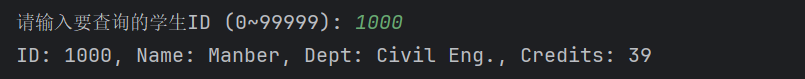
\includegraphics[width=11cm]{./images/20.查询ID.png}
		\caption{查询ID}
	\end{figure}
	
	\begin{figure}[H]
		\centering
		
\includegraphics[width=11cm]{./images/21.查询ID错误.png}
		\caption{查询ID错误-未找到}
	\end{figure}
	
	\subsubsection{学生课程信息查询}
	\begin{enumerate}
		\item 若找到学生信息,用户可输入 1 以查询该学生所修读的所有课程信息,包括:
		\begin{itemize}
			\item 课程 ID
			\item 上课年份
			\item 上课学期
			\item 课程名称
			\item 开课院系
			\item 成绩等级
			\item 课程学分数
		\end{itemize}
		\item 若用户输入 0,则停止查询。
	\end{enumerate}
	
	\begin{lstlisting}[language=java, title=学生课程信息查询, tabsize=4]
		private static void searchStudentCourses(Connection conn, int studentId) throws SQLException {
			Scanner scanner = new Scanner(System.in);
			System.out.print("输入1查看该学生修读的课程信息,输入0退出: ");
			if (scanner.nextInt() != 1) return;
			scanner.nextLine();
			
			String query = "SELECT takes.course_id, year, semester, title, dept_name, grade, credits FROM takes JOIN course ON takes.course_id = course.course_id WHERE ID = ?";
			try (PreparedStatement stmt = conn.prepareStatement(query)) {
				stmt.setInt(1, studentId);
				ResultSet rs = stmt.executeQuery();
				boolean found = false;
				while (rs.next()) {
					found = true;
					System.out.println("课程ID: " + rs.getString("course_id") + ", 年份: " + rs.getInt("year") + ", 学期: " + rs.getString("semester") + ", 课程名: " + rs.getString("title") + ", 院系: " + rs.getString("dept_name") + ", 成绩: " + rs.getString("grade") + ", 学分: " + rs.getInt("credits"));
				}
				if (!found) {
					System.out.println("该学生没有修读课程。");
				} else {
					calculateGPA(conn, studentId);
				}
			}
		}
	\end{lstlisting}
	
	运行结果如下图所示(多余部分省略):
	
	\begin{figure}[H]
		\centering
		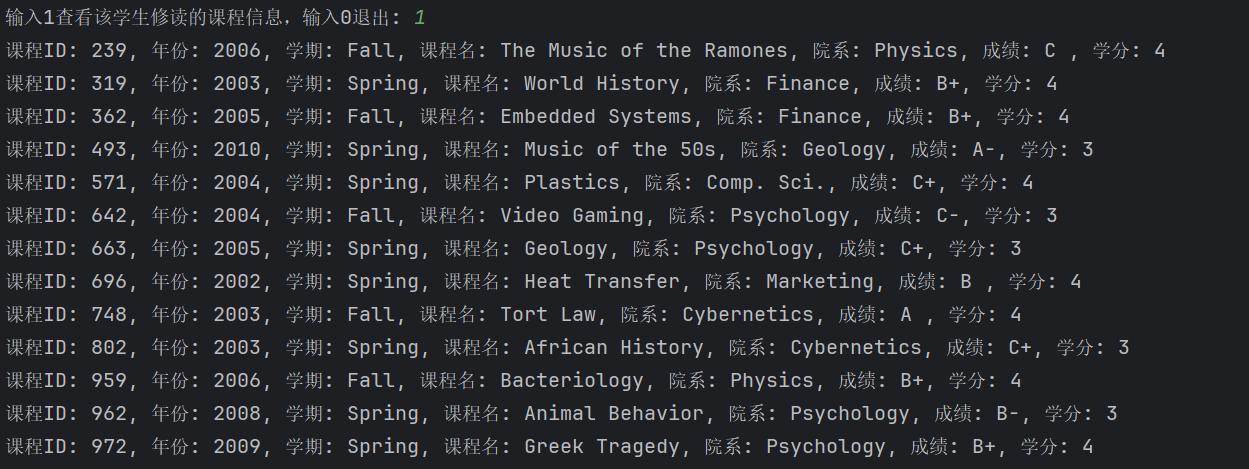
\includegraphics[width=13cm]{./images/22.查询课程.png}
		\caption{查询课程信息}
	\end{figure}
	
	\subsubsection{计算平均绩点(GPA)}
	\begin{enumerate}
		\item 若学生有修读课程,用户可输入 1 计算该学生的平均绩点(GPA)并显示。
		\item 若用户输入 0,则停止查询。
	\end{enumerate}
	
	\mybox[blue]{这里采用 SUM(学分*绩点)/ SUM(学分) 的方法来计算平均绩点}
	
	\begin{lstlisting}[language=java, title=计算平均绩点(GPA), tabsize=4]
		private static void calculateGPA(Connection conn, int studentId) throws SQLException {
			Scanner scanner = new Scanner(System.in);
			System.out.print("输入1计算该学生的平均绩点,输入0退出: ");
			if (scanner.nextInt() != 1) return;
			scanner.nextLine();
			
			String query = "SELECT grade_point, credits FROM (takes JOIN course ON takes.course_id = course.course_id) JOIN gpa ON gpa.grade = TRIM(takes.grade) WHERE ID = ?";
			try (PreparedStatement stmt = conn.prepareStatement(query)) {
				stmt.setInt(1, studentId);
				ResultSet rs = stmt.executeQuery();
				double totalPoints = 0;
				int totalCredits = 0;
				while (rs.next()) {
					float grade_point = rs.getFloat("grade_point");
					int credits = rs.getInt("credits");
					totalCredits += credits;
					totalPoints += grade_point * credits;
				}
				if (totalCredits == 0) {
					System.out.println("该学生无可计算绩点的课程。");
				} else {
					double gpa = totalPoints / totalCredits;
					System.out.printf("该学生的平均绩点(两位小数)为: %.2f\n", gpa);
				}
			}
		}
	\end{lstlisting}
	
	\begin{tcolorbox}[title = {TRIM函数的使用}, colback = blue!25!white, colframe = blue!75!black]
		在这里我使用了TRIM函数,因为在takes表格中,A,B,C等绩点,存储格式是"A ","B "这样会导致JOIN的时候由于条件不符合而被忽略,所以使用TRIM函数来取消空格带来的影响
	\end{tcolorbox}
	
	\begin{figure}[H]
		\centering
		
\includegraphics[width=11cm]{./images/23.计算平均绩点.png}
		\caption{计算平均绩点}
	\end{figure}
	
	\subsubsection{异常处理要求}
	\begin{enumerate}
		\item 连接数据库成功后,所有数据库操作需捕获异常并进行处理,程序不应因异常停止运行。
		\item 若用户输入不合法数据,需给出相应提示,并允许重新输入。
	\end{enumerate}
	
	所有的执行过程都用try-catch来包裹,可以做出自定义的提示,而不是报错中断,
	
	\mybox[red]{具体代码与运行结果上面已经展示,此处不再展示}
	
	\section{存在的问题及解决方案}
	在实验过程中,可能会遇到以下问题及相应的解决方案:
	\begin{itemize}
		\item \textbf{数据库连接失败}:
		\begin{itemize}
			\item 确保 MySQL 服务器已启动。
			\item 检查 JDBC URL、用户名和密码是否正确。
			\item 确保 MySQL 允许远程连接(修改 my.cnf 或 my.ini 配置文件)。
		\end{itemize}
		\item \textbf{SQL 语句执行错误}:
		\begin{itemize}
			\item 使用 PreparedStatement 避免 SQL 注入问题。
			\item 通过日志调试 SQL 语句是否正确执行。
		\end{itemize}
		\item \textbf{编码问题(如中文乱码)}:
		\begin{itemize}
			\item 在数据库连接 URL 末尾添加 useUnicode=true\&characterEncoding=UTF-8。
			\item 设置 MySQL 数据库的字符集为 UTF-8。
		\end{itemize}
		\item \textbf{驱动加载失败}:
		\begin{itemize}
			\item 确保 MySQL JDBC 驱动包已正确导入。
			\item 使用 `Class.forName("com.mysql.cj.jdbc.Driver")` 确保驱动正确加载。
		\end{itemize}
		\item \textbf{takes与gpa里的grade格式不一致}:
		\begin{itemize}
			\item 在takes表格中,A,B,C等绩点,存储格式是"A ","B "
			\item 在gpa表格中,A,B,C等绩点,存储格式是"A","B"
			\item 使用TRIM来消除空格带来的影响。
		\end{itemize}
	\end{itemize}
	
	\section{实验小结}
	通过本次实验,学生学习了 JDBC 技术的基础知识,并成功实现了 Java 应用程序与 MySQL 数据库的连接与交互。实验过程中遇到的问题,如数据库连接失败、SQL 语句错误等,都得到了有效解决。通过本实验,学生对数据库操作有了更深入的理解,并为后续的数据库应用开发打下了良好的基础。此外,学生还认识到了编写健壮、安全的数据库交互代码的重要性,为后续的编程实践提供了宝贵的经验。
	
	
\end{document}